\section{Rappels de C}

\subsubsection{Types en C}
Dans le langage C les types contrôlent : la \textbf{taille en mémoire} que la
donnée occupe, et le \textbf{comportement de diverses opérations}. Tout type a
une taille que l'on peut récupérer avec \verb|sizeof(type)|.

\begin{remark}
  Le type n'existe \textit{qu'au moment de la compilation}, il n'y a pas de type
  dynamique. Nothing in the running program carries a tag saying ``I am an
  \verb|int|''. A value is a pile of bytes, and the type is the compilateur's
  private record of how to read them --- which is why a wrong cast is silent
  and a wrong \verb|printf| format prints garbage instead of raising an error.
\end{remark}

\begin{center}
\begin{tabular}{llll}
  \toprule
  Type & Typical size & Holds & Note \\
  \midrule
  \verb|char|      & 1 octet  & a character / a small integer & the unit of \verb|sizeof| \\
  \verb|int|       & souvent 4 & a decimal integer             & not fixed by the standard \\
  \verb|long long| & souvent 8 & a wide integer                & literal suffix \verb|LL| \\
  \verb|void|      & 1 mais mal défini & nothing             & used as a return type, and as \verb|void *| \\
  \verb|T *|       & 8 on x86-64 & an address                & any type of pointeur, whatever \verb|T| is \\
  \bottomrule
\end{tabular}
\end{center}

The word ``souvent'' is the point: \verb|int| is \textit{souvent 4} and
\verb|long long| \textit{souvent 8}, because the sizes are properties of the
implementation, not of the language. Only \verb|sizeof(char)| is pinned to $1$,
since it \textit{defines} the unit.\\

On peut rajouter des \textbf{modificateurs} (\textit{modifiers}) pour changer le
comportement. They are added in front of a type: \verb|signed| and
\verb|unsigned| change how the same bytes are interpreted and therefore how
comparison, division and overflow behave, and \verb|const| marks the object as
non-modifiable.

\subsubsection{Variable}
\begin{definition}[Variable]
  Définir une variable en C c'est \textbf{réserver de la mémoire}. Il faut donc
  le type (pour savoir \textit{combien} de mémoire) et on peut rajouter une
  valeur initiale.
\end{definition}

\begin{lstlisting}[language=C]
int a ;
char b = 42 ;
long long c, d = factoriel(15);
int e, f=12, g=33, h;
\end{lstlisting}

On modifie une variable avec \verb|=|, comme \verb|b = 42;| ou \verb|x = y;|.
La \textbf{durée de vie} (\textit{lifetime}) d'une variable est celle du bloc
où elle est définie, sa mémoire peut être utilisée pour autre chose avant ou
après. Nothing zeroes it on the way in and nothing preserves it on the way out.

\subsubsection{Variables --- où sont-elles stockées}
This is the section the next chapter is built on. En général, les compilateurs
C font les choix suivants :

\begin{center}
\begin{tabular}{lll}
  \toprule
  Situation & Storage & Why \\
  \midrule
  la durée de vie est très courte & un \textbf{registre} & pour qu'elle n'existe \\
  et le compilateur peut          &                       & que dans un registre \\
  optimiser la variable           &                       & \\
  \addlinespace
  la variable est \textbf{globale} & un \textbf{segment déclaré} & il n'existe qu'une version \\
                                   & \textbf{dans l'assembleur}  & de cette variable \\
                                   &                             & (one for the whole program) \\
  \addlinespace
  la variable est déclarée & la \textbf{pile} & elle peut exister plusieurs fois \\
  \textbf{dans une fonction} &                & (appels récursifs), il faut donc \\
                             &                & lui allouer de la mémoire \\
                             &                & pour chaque appel \\
  \bottomrule
\end{tabular}
\end{center}

Which segment a global lands in is decided by two independent bits --- is it
modifiable, and is it initialised:

\begin{center}
\begin{tabular}{lll}
  \toprule
  Modifiable? & Initialised? & Section \\
  \midrule
  yes & yes & \verb|.data| \\
  yes & no  & \verb|.bss| \\
  no  & --- & \verb|.rodata| \\
  \bottomrule
\end{tabular}
\end{center}

\begin{figure}[h!]
  \centering
  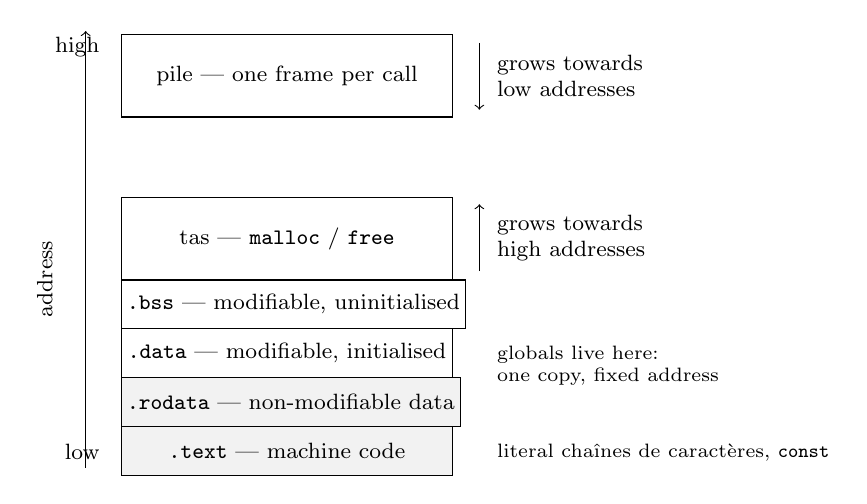
\begin{tikzpicture}[font=\footnotesize]
    \tikzset{seg/.style={draw, minimum width=4.2cm, minimum height=0.62cm,
             anchor=south west, align=center, inner sep=2pt}}
    \node[seg, fill=black!5] at (0,0.00) {\texttt{.text} --- machine code};
    \node[seg, fill=black!5] at (0,0.62) {\texttt{.rodata} --- non-modifiable data};
    \node[seg]               at (0,1.24) {\texttt{.data} --- modifiable, initialised};
    \node[seg]               at (0,1.86) {\texttt{.bss} --- modifiable, uninitialised};
    \node[seg, minimum height=1.05cm] at (0,2.48) {tas --- \texttt{malloc} / \texttt{free}};
    \node[seg, minimum height=1.05cm] at (0,4.55) {pile --- one frame per call};
    \draw[dashed] (0,3.53) -- (4.2,3.53);
    \draw[dashed] (0,4.55) -- (4.2,4.55);
    \draw[->] (4.55,2.60) -- (4.55,3.45);
    \node[right, align=left] at (4.65,3.02) {grows towards\\high addresses};
    \draw[->] (4.55,5.50) -- (4.55,4.65);
    \node[right, align=left] at (4.65,5.08) {grows towards\\low addresses};
    \node[left] at (-0.15,0.31) {low};
    \node[left] at (-0.15,5.45) {high};
    \draw[->] (-0.45,0.10) -- (-0.45,5.65);
    \node[rotate=90, anchor=south] at (-0.75,2.5) {address};
    \node[right, align=left, font=\scriptsize] at (4.65,1.40)
      {globals live here:\\one copy, fixed address};
    \node[right, align=left, font=\scriptsize] at (4.65,0.30)
      {literal chaînes de caractères, \texttt{const}};
  \end{tikzpicture}
\end{figure}

\begin{example}[Divers stockages de variables]
  This example puts one global, one addressed local and one optimised-away
  local in the same function and shows the assembly the compilateur emits.
  \begin{lstlisting}[language=C]
int globale = 123;

int f() {
  int locale = 456;
  int inlinee = 1+g(&locale);
  return inlinee;
}
  \end{lstlisting}
  \begin{lstlisting}[language=gas]
  .text
  .globl f
f:
  subq $24, %rsp
  movl $456, 12(%rsp)    ;;; locale dans 12(%rsp)
  leaq 12(%rsp), %rdi
  call g@PLT
  addl $1, %eax          ;;; inlinee dans %eax
  addq $24, %rsp
  ret
  .globl globale
  .data
globale:                 ;;; globale dans section data car modifiable
  .long 123              ;;; et initialisee
  ;;; dans une section bss si modifiable non initialisee
  ;;; dans une section rodata si non modifiable
  \end{lstlisting}
  Reading the three variables off the listing:
  \begin{center}
  \begin{tabular}{llll}
    \toprule
    Variable & Durée de vie & Where & Evidence \\
    \midrule
    \verb|globale| & the whole program & \verb|.data| & \verb|globale: .long 123| \\
    \verb|locale|  & one call to \verb|f| & the pile, at \verb|12(%rsp)| & \verb|movl $456, 12(%rsp)| \\
    \verb|inlinee| & one call to \verb|f| & the registre \verb|%eax| & \verb|addl $1, %eax| \\
    \bottomrule
  \end{tabular}
  \end{center}
  The \verb|subq $24, %rsp| / \verb|addq $24, %rsp| pair is the frame being
  opened and closed; \verb|locale| occupies four of those twenty-four bytes.
\end{example}

\begin{remark}
  \verb|locale| and \verb|inlinee| are both locals of the same function and yet
  they are stored differently. The discriminating fact is in the source code: the
  program writes \verb|&locale|, so \verb|locale| must have an address, and the
  compilateur is forced to give it a slot on the pile --- hence
  \verb|leaq 12(%rsp), %rdi|, which hands that address to \verb|g|.
  \verb|inlinee| is never addressed, is read once, and is therefore allowed to
  exist only in \verb|%eax|. ``Having an address'' is exactly the valeur gauche
  notion of the next subsection, and it is what decides registre versus pile.
\end{remark}

\subsubsection{Fonctions}
Syntaxe générale :
\begin{lstlisting}[language=C]
type_retour nom_fonction(type1 arg1, type2 arg2) {
   /// code de la fonction
   return valeur_retour;
}
\end{lstlisting}
Précisions : on met usuellement \verb|type_retour = void| si la fonction ne
renvoie rien, et le \verb|return| est facultatif (mais on ne sait alors pas ce
que la fonction renvoie).

\begin{example}
  \begin{lstlisting}[language=C]
int produit(int a, int b) { return a*b; }
int life() { return 42; }
void set(int v) { x=v; }
  \end{lstlisting}
\end{example}

\subsubsection{Expressions}
Les expressions en C sont (entre autres) composées :
\begin{itemize}
  \item des \textbf{constantes} \verb|42|, \verb|0xA2|, \verb|'H'| que l'on
    peut typer (p.~ex.\ \verb|42LL| est $42$ en \verb|long long|);
  \item des \textbf{variables};
  \item de \textbf{sous-expressions parenthésées};
  \item des \textbf{appels de fonctions};
  \item de diverses \textbf{opérations binaires infixes} : \verb|+|, \verb|-|,
    \verb|*|, \verb|/|, \verb|<|, \verb|>|, \verb|<=|, \verb|>=|, \verb|=|,
    \verb|==|, \verb|%|;
  \item de divers \textbf{opérateurs unaires} : \verb|!|, \verb|~|, \verb|-|,
    \verb|*|, \verb|&|, \verb|++|, \verb|--|.
\end{itemize}
Toute expression a un type qui définit la place nécessaire et le comportement.

\begin{remark}
  \verb|=| appears in the list of \textit{opérations binaires}, not in a separate
  list of statements. Assignment is an expression whose value is the value
  assigned, which is what makes \verb|y=(x=42*f(3,5*g(2)))| legal: the inner
  assignment to \verb|x| yields a value, and that value is then stored in
  \verb|y|.
\end{remark}

\begin{example}[Four expressions]
  \begin{center}
  \begin{tabular}{ll}
    \toprule
    Expression & What it does \\
    \midrule
    \verb|y=(x=42*f(3,5*g(2)))| & nested calls; the assignment to \verb|x| returns a value \\
    \verb|x=(1+(2<3))| & \verb|2<3| evaluates to $1$, so \verb|x| becomes $2$ \\
    \verb|0.+1/2| & \verb|1/2| is \textit{integer} division, i.e.\ $0$; the result is $0.0$ \\
    \verb|(0.+1)/2| & \verb|0.+1| is a \verb|double|, so the division is real: $0.5$ \\
    \bottomrule
  \end{tabular}
  \end{center}
  The last two differ only by a pair of parentheses and by a factor of
  infinity in the answer, because the type of a sub-expression --- not the type
  of the variable being assigned --- decides which division is compiled.
\end{example}

\subsubsection{Structures de contrôle}
\begin{lstlisting}[language=C]
while(condition) fairequelquechose

if(condition) fairequelquechose
if(condition) fairequelquechose else fairequelquechose
\end{lstlisting}
Si \verb|fairequelquechose| est composé de plusieurs instructions il faut les
mettre entre accolades. Une condition est \textbf{vraie} si en l'évaluant on
obtient une valeur \textit{différente de} $0$. There is no separate boolean
type to satisfy.

\begin{example}[Collatz]
  \begin{lstlisting}[language=C]
int n = 0; while(n<42) n++;
while(n!=1) {
  if(n%2)        /// teste la parite car n%2=0 <==> n est pair
    n = 3*n+1 ;  /// n est forcement pair maintenant
  n /= 2;
}
  \end{lstlisting}
  The condition \verb|n%2| is used directly as the test: it is $0$ when
  \verb|n| is even and $1$ when it is odd, and no comparison against a boolean
  is written. The comment records the loop's invariant --- after the
  \verb|if| body, \verb|n| is necessarily even, so the unconditional
  \verb|n /= 2| is exact.
\end{example}

\subsection{Pointeurs}
\subsubsection{Valeur gauche}
\begin{definition}[Valeur gauche]
  Une \textbf{valeur gauche} (\textit{left-value}) c'est une valeur qui peut
  être à gauche dans un \verb|=|. En C une valeur gauche c'est une valeur qui
  est \textbf{stockée quelque part en mémoire} (et qui a un type). Autrement
  dit, une valeur gauche c'est quelque chose qui \textbf{a une adresse en
  mémoire}.
\end{definition}

\begin{lstlisting}[language=C]
int a;
a = 42 ; /// autorise
42 = a ; /// interdit, on ne peut pas modifier 42
\end{lstlisting}
\verb|a| est une valeur gauche mais pas \verb|42|. There is no memory cell
called ``\,$42$\,'' to write into.

\subsubsection{Pointeur}
\begin{definition}[Pointeur]
  Un \textbf{pointeur} (\textit{pointer}) est un objet qui stocke l'adresse
  mémoire d'un certain type :
  \begin{itemize}
    \item \verb|T* p| déclare un pointeur \verb|p| vers un objet de type \verb|T|;
    \item \verb|&a| récupère l'adresse d'un objet \verb|a|;
    \item \verb|*p| renvoie l'objet de type \verb|T| pointé par \verb|p|;
    \item \verb|*p| est une valeur gauche car \verb|*p| est stocké à
      l'adresse \verb|p|.
  \end{itemize}
\end{definition}

\begin{remark}
  \verb|&| is the \textit{address-of} or \textit{referencing} operator and
  \verb|*| is the \textit{dereferencing} or \textit{indirection} operator:
  taking \verb|&a| is référencer, evaluating \verb|*p| is déréférencer. The
  operators themselves are unambiguous --- \verb|&| goes from an object to its
  address, \verb|*| goes from an address to the object --- and the two names
  are easy to swap, so read the symbols and not the names.
\end{remark}

\begin{lstlisting}[language=C]
int a, b ;
int * t ;  /// int* c'est un type de pointeur vers un int
t = &a ;   /// t stocke maintenant l'adresse de a
*t = 42 ;
t = &b ; *t = 17;  /// a vaut 42 et b vaut 17
\end{lstlisting}

\begin{figure}[h!]
  \centering
  \begin{tikzpicture}[font=\footnotesize]
    \tikzset{cell/.style={draw, minimum width=1.7cm, minimum height=0.62cm}}
    \node[cell] (a) at (0,0)   {\texttt{42}};
    \node[cell] (b) at (2.6,0) {\texttt{17}};
    \node[above=2pt of a] {\texttt{int a}};
    \node[above=2pt of b] {\texttt{int b}};
    \node[cell] (t) at (1.3,-1.7) {\texttt{\&b}};
    \node[below=2pt of t] {\texttt{int *t}};
    \draw[->, thick]  (t.north) -- ++(0,0.45) -| (b.south);
    \draw[->, dashed] (t.north) -- ++(0,0.45) -| (a.south);
    \node[right, align=left, font=\scriptsize] at (3.9,-0.85)
      {dashed: after \texttt{t = \&a}\\solid: after \texttt{t = \&b}\\
       \texttt{*t} is whichever cell\\the arrow ends in};
  \end{tikzpicture}
\end{figure}

Two identities follow directly from the definition, and they are the ones to
recite in an exam.

\begin{prop}[Allers-retours]
  Quand \verb|a| est une valeur gauche, alors
  \begin{center}
    \verb|*(&a) == a|,
  \end{center}
  car \verb|&a| récupère l'adresse de \verb|a| et \verb|*| récupère ensuite la
  valeur à cette adresse. De même si \verb|a| pointe vers quelque chose alors
  \begin{center}
    \verb|&(*a) == a|,
  \end{center}
  car \verb|*a| crée une valeur gauche stockée à l'adresse \verb|a| et \verb|&|
  récupère ensuite l'adresse de la valeur gauche.
\end{prop}

\begin{remark}
  \verb|*a| est \textbf{toujours} une valeur gauche, \verb|&a| ne l'est
  \textbf{jamais}. The asymmetry is the whole content of the previous subsection: \verb|*a|
  names a cell, whereas \verb|&a| is a computed address that is not itself
  stored anywhere. Hence \verb|*p = 42| compiles and \verb|&a = 42| does not.
\end{remark}

\subsubsection{Arithmétique de pointeurs}
Le type des pointeurs change le comportement de l'arithmétique. For
\verb|p|, \verb|p1|, \verb|p2| of type \verb|T*| and \verb|i| an integer:
\begin{align*}
  p + i &\;\Longleftrightarrow\; p + \mathtt{sizeof}(T) \times i, \\
  p - i &\;\Longleftrightarrow\; p - \mathtt{sizeof}(T) \times i, \\
  p_1 - p_2 &\;\Longleftrightarrow\; (p_1 - p_2) \,/\, \mathtt{sizeof}(T)
    \qquad \text{for } p_1,\, p_2 \text{ of the same type } \text{\texttt{T*}}, \\
  \text{\texttt{p++}} &\;\Longleftrightarrow\; p = p + 1.
\end{align*}
Les opérations qui n'ont pas de sens échouent : $p_1 + p_2$, $p_1 * p_2$,
etc. Adding two addresses names nothing, whereas subtracting two addresses of
the same type names a count of elements.

\begin{remark}
  The scaling is silent. Si \verb|t| pointe vers un entier 4 octets,
  \verb|t+1| vers l'entier \textit{d'après} qui est 4 octets plus loin. The
  source code reads \verb|t+1| and the machine computes
  $\verb|t| + 4$. This is also why \verb|void *| arithmetic is ill-defined:
  \verb|sizeof(void)| is ``$1$ mais mal défini''.
\end{remark}

\subsubsection{Tableaux}
Les tableaux sont \textbf{presque que des pointeurs} :

\begin{lstlisting}[language=C]
int t[5] = {1,2,3,4,5} ;
int * x = t;
*x = 1 ;       /// modifie t[0]
*(x+2) = 2 ;   /// modifie t[2]
\end{lstlisting}

\begin{prop}[L'indexation est du sucre syntaxique]
  En C, \verb|t[i]| est du \textbf{sucre syntaxique} (\textit{syntactic sugar})
  pour
  \[ \verb|*(t+i)|. \]
\end{prop}

\begin{remark}
  \verb|+| is commutative, so \verb|*(t+i)| is \verb|*(i+t)|. On peut
  d'ailleurs écrire \verb|4[t]| plutôt que \verb|t[4]|. It compiles. The
  bracket is therefore not a primitive operation on a special ``array'' object
  but a règle de réécriture on a pointeur and an integer.
\end{remark}

L'initialisation de la forme \verb|int t[10]| marche quand on connaît la taille
du tableau. Cela réserve $10 \times \verb|sizeof(int)|$ octets. Si on ne
connaît \textit{pas} la taille du tableau à la compilation il faut demander de
la mémoire à l'OS. Il y a une fonction dans la libC qui gère l'allocation
mémoire : \verb|malloc|.

\begin{lstlisting}[language=C]
int * t = malloc(40) ;
  /// 40 octets, soit 10 int de taille 4

t = malloc( 10 * sizeof(int) ) ; /// autre maniere
/// de demander la meme chose
\end{lstlisting}

\begin{remark}
  The two calls request the same thing, but only the second survives a change
  of architecture: the literal \verb|40| silently assumes
  \verb|sizeof(int) == 4|, which the table of types above gives as only
  \textit{souvent} true. Write the \verb|sizeof| form.
\end{remark}

\subsubsection{Chaînes de caractères}
En C, les caractères sont de type \verb|char| et les \textbf{chaînes de
caractères} (\textit{strings}) sont simplement des tableaux de caractères, et
des pointeurs \verb|char*|. Une chaîne de la forme \verb|"machaine"| dans le
programme C est une valeur de type \verb|const char *|.

\begin{notation}
  Par convention, une chaîne de caractères se termine par le caractère
  \verb|'\0'| dont la valeur numérique est $0$. Nothing else records the
  length: the terminator \textit{is} the length.
\end{notation}

\begin{lstlisting}[language=C]
const char * s = "Hello World!"; /// C rajoute un '\0'
int len = 0 ;
while(s[len])  /// s'arrete quand s[len] vaut 0 = '\0'
  len++;
s[2] = '?' ;   /// que va faire cette ligne ?
\end{lstlisting}

\begin{remark}
  The loop needs no comparison: \verb|s[len]| is itself the condition, and it
  is false exactly on the terminator, since a condition is true when it differs
  from $0$ and \verb|'\0'| \textit{is} $0$. On exit, \verb|len| is the number of
  characters before the terminator.
\end{remark}

\begin{remark}
  The listing's last line is left as a question. Two independent things are
  wrong with \verb|s[2] = '?'|. The type of \verb|s| is \verb|const char *|, so
  the pointed-to object is declared non-modifiable and the compilateur objects.
  And by the storage rules above, non-modifiable data goes in \verb|.rodata|, a
  section the loader maps read-only --- so forcing the write past the
  compilateur gets it refused by the hardware at run time rather than executed.
\end{remark}

\subsection{Bibliothèque C}
\begin{definition}[libC]
  La \textbf{libC} (pour C library et donc bibliothèque C) est un ensemble de
  fonctions qui permettent à C d'interagir avec l'OS \textit{quel que soit}
  l'OS. It is the portability layer: the C program calls libC, and libC calls
  whichever system interface the platform actually has.
\end{definition}

La libC contient beaucoup de fonctions, vous devez en connaître 4 :
\begin{center}
\begin{tabular}{ll}
  \toprule
  Function & Role \\
  \midrule
  \verb|malloc| & alloue de la mémoire (déjà vue) \\
  \verb|free|   & libère de la mémoire allouée par \verb|malloc| \\
  \verb|printf| & affiche sur la sortie standard \\
  \verb|scanf|  & lit sur l'entrée standard \\
  \bottomrule
\end{tabular}
\end{center}

\subsubsection{printf}
La fonction \verb|printf| prend un nombre arbitraire de paramètres et le premier
paramètre est un \textbf{format} de type chaîne de caractères. The format is
copied to the output verbatim except at the \verb|%| placeholders, each of
which consumes one further argument.

\begin{example}
  \begin{lstlisting}[language=C]
printf("Hello World!");
printf("%d",42);
printf("%s","Hello World");
printf("a=%d / b=%d / chaine %s", 1, 2, "coucou");
\end{lstlisting}
  The last line is the general case: several arguments interleaved with literal
  text, consumed left to right in the order the placeholders appear.
\end{example}

\paragraph{Formats utiles}
Voici les formats qui peuvent être utiles dans ce cours :
\begin{center}
\begin{tabular}{lll}
  \toprule
  Format & Argument & Size of the argument \\
  \midrule
  \verb|%d|   & entier décimal sous forme de \verb|int| & souvent 4 octets \\
  \verb|%lld| & entier décimal sous forme de \verb|long long| & 8 octets \\
  \verb|%s|   & chaîne de caractères (pointeur vers le premier caractère) & 8 octets \\
  \verb|%c|   & affiche un unique caractère & --- \\
  \verb|%p|   & affiche l'adresse d'un pointeur & 8 octets \\
  \bottomrule
\end{tabular}
\end{center}

\begin{remark}
  \textbf{Attention} : pour \verb|printf| il faut faire attention à ce que
  \textit{les tailles des types soient les bonnes}. \verb|printf| is variadic:
  it cannot inspect what it was handed, so it reads as many bytes off the
  argument area as the format tells it to. Passing a \verb|long long| to
  \verb|%d| or an \verb|int| to \verb|%lld| makes \verb|printf| read the wrong
  number of bytes for that placeholder and print garbage; on ABIs that pass
  variadic arguments on the pile it additionally shifts every later argument.
  The compilateur has no type to check against. This is the practical face of
  ``le type n'existe qu'au moment de la compilation''.
\end{remark}

\subsubsection{scanf}
La fonction \verb|scanf| est similaire à \verb|printf| excepté qu'elle
\textit{lit}. Les arguments ne sont pas tout à fait les mêmes car \verb|printf|
prend des \textbf{valeurs}, \verb|scanf| doit prendre des \textbf{pointeurs} :
\begin{itemize}
  \item pour lire une chaîne de caractères, ça ne change pas le type, on passe
    un pointeur où l'on veut que \verb|scanf| stocke la chaîne (comme
    \verb|printf|);
  \item pour lire un entier, on passe un pointeur où stocker l'entier.
\end{itemize}

\begin{lstlisting}[language=C]
char chaine_lue[100] ;
int entier_lu ;
scanf("%s %d",chaine_lue, &entier_lu);
/// en lisant une chaine avec %s scanf s'arrete a la premiere espace ' ',
/// tabulation '\t' ou retour a la ligne '\n'
/// avec %d l'entier doit etre decimal (%i pour octal ou hexadecimal)
\end{lstlisting}

\begin{remark}
  \verb|chaine_lue| is passed bare and \verb|entier_lu| is passed as
  \verb|&entier_lu|. That is not an inconsistency: the array name already
  \textit{is} the address of its first element, so it is already the pointeur
  \verb|scanf| wants, whereas \verb|entier_lu| is an \verb|int| and needs the
  \verb|&|. Reading \verb|t[i]| as \verb|*(t+i)| makes this automatic.
\end{remark}

\begin{remark}
  Two behaviours of the format worth keeping. First, \verb|%s| s'arrête à la
  première espace \verb|' '|, tabulation \verb|'\t'| ou retour à la ligne
  \verb|'\n'|, so it reads one word and not one line. Second, avec \verb|%d|
  l'entier doit être \textit{décimal} (\verb|%i| pour octal ou hexadécimal, as
  well as decimal).
\end{remark}

\subsection{Tableaux}
\subsubsection{Tableaux 2D}
Une solution avec \texttt{malloc} : an array of pointeurs to arrays.

\begin{lstlisting}[language=C]
int ** t ;
/// un pointeur vers des
/// pointeurs vers des entiers

t = malloc( sizeof(int*) * 10 ) ;
/// attention sizeof(int*) !

int i = 0;
while(i<10) {
  t[i] = malloc( sizeof(int) * 10 ) ;
  i++;
}
\end{lstlisting}

\begin{figure}[h!]
  \centering
  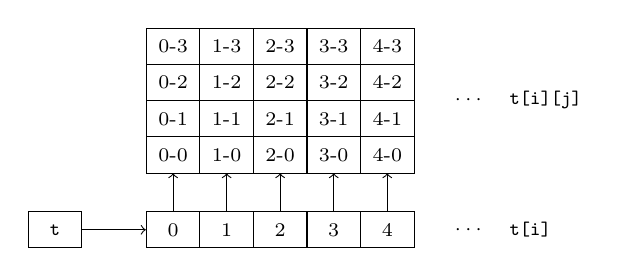
\begin{tikzpicture}[font=\scriptsize]
    \tikzset{c/.style={draw, minimum width=0.68cm, minimum height=0.46cm, inner sep=1pt}}
    \foreach \i in {0,...,4} {
      \node[c] (p\i) at (\i*0.68,0) {\i};
      \foreach \j in {0,...,3} {
        \node[c] at (\i*0.68, 0.95+\j*0.46) {\i-\j};
      }
      \draw[->] (\i*0.68,0.23) -- (\i*0.68,0.72);
    }
    \node at (3.75,0) {$\cdots$};
    \node at (3.75,1.65) {$\cdots$};
    \node[c] (root) at (-1.5,0) {\texttt{t}};
    \draw[->] (root.east) -- (p0.west);
    \node[right] at (4.15,1.65) {\texttt{t[i][j]}};
    \node[right] at (4.15,0)    {\texttt{t[i]}};
  \end{tikzpicture}
\end{figure}

\begin{remark}
  \textit{Attention} \verb|sizeof(int*)| in the first \verb|malloc|: the outer
  allocation holds \textit{pointeurs}, 8 bytes each, not integers. Writing
  \verb|sizeof(int)| there would reserve half the memory needed and corrupt the
  spine of the structure.
\end{remark}

\begin{remark}
  C'est le même fonctionnement en OCaml et en Python : un tableau
  multidimensionnel est un \textbf{tableau de tableaux}. The rows are separate
  allocations, so they need not be contiguous with one another and need not
  even have the same length.
\end{remark}

\subsubsection{Tableaux linéarisés}
The other solution is the built-in multidimensional array, which is not an
array of arrays at all.

\begin{lstlisting}[language=C]
int t[99][88][77] ; /// en fait c'est un tableau de taille 99x88x77

int i =3, j=4, k=5;
t[i][j][k] /// est remplace par *(t+i*88*77+j*77+k)
\end{lstlisting}

A single block of $99 \times 88 \times 77$ integers is reserved, and the
indices are folded into one offset. The compilateur turns
\begin{center}
  \verb|t[i][j][k]| $\longrightarrow$ \verb|*(t + i*88*77 + j*77 + k)|,
\end{center}
where the offset is counted in \textit{elements} --- the scaling by
\verb|sizeof(int)| is then supplied by the arithmétique de pointeurs of the
previous subsection. Note which dimensions appear: the first, $99$, does not, while
$88$ and $77$ do.

\begin{figure}[h!]
  \centering
  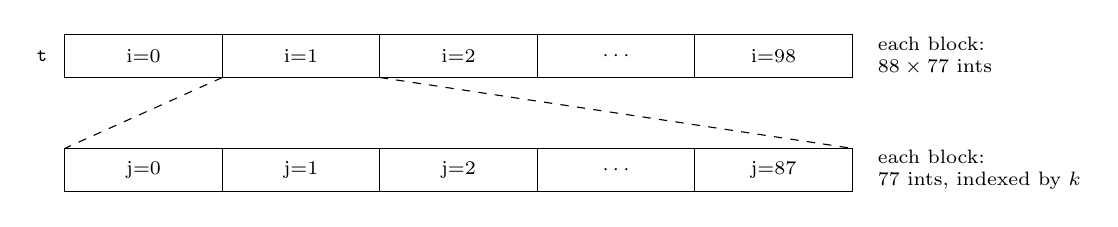
\begin{tikzpicture}[font=\scriptsize]
    % top strip: the i-blocks
    \draw (0,0) rectangle (10,0.55);
    \foreach \x in {2,4,6,8} \draw (\x,0) -- (\x,0.55);
    \foreach \x/\l in {1/{i=0}, 3/{i=1}, 5/{i=2}, 7/{$\cdots$}, 9/{i=98}}
      \node at (\x,0.275) {\l};
    \node[left] at (-0.1,0.275) {\texttt{t}};
    \node[right, align=left] at (10.2,0.275) {each block:\\$88\times 77$ ints};
    % guides
    \draw[dashed] (2,0) -- (0,-0.9);
    \draw[dashed] (4,0) -- (10,-0.9);
    % bottom strip: the j-blocks inside one i-block
    \draw (0,-1.45) rectangle (10,-0.9);
    \foreach \x in {2,4,6,8} \draw (\x,-1.45) -- (\x,-0.9);
    \foreach \x/\l in {1/{j=0}, 3/{j=1}, 5/{j=2}, 7/{$\cdots$}, 9/{j=87}}
      \node at (\x,-1.175) {\l};
    \node[right, align=left] at (10.2,-1.175) {each block:\\$77$ ints, indexed by $k$};
  \end{tikzpicture}
\end{figure}

\begin{remark}
  Le type tableau multidimensionnel est un pointeur avec l'information
  additionnelle des dimensions (sauf la première) et un peu compliqué
  à comprendre. Il vaut mieux éviter de faire des choses compliquées avec. The
  first dimension is absent because it is never needed to compute an offset
  --- only the strides below a given index matter.
\end{remark}

\begin{example}[Passing a slice]
  \begin{lstlisting}[language=C]
void f(int a[][77]) { a[2][3] = 42 ; } /// a est un pointeur
int (*x)[88][77] = t;
f(x[1]); /// calcule x+1*sizeof(int[88][77]) = 88*77*4
  \end{lstlisting}
  The parameter \verb|int a[][77]| is a pointeur that remembers the stride
  $77$, which is all \verb|a[2][3]| needs: the offset is $2 \times 77 + 3$
  elements. The variable \verb|x| is a pointeur to an \verb|int[88][77]|, so
  \verb|x[1]| advances by one whole $88 \times 77$ slab --- the comment records
  the arithmetic as $88 \times 77 \times 4$ bytes, the factor $4$ being
  \verb|sizeof(int)|.
\end{example}

\begin{conclusion}
  The two constructions have the same indexing syntax and nothing else in
  common. \verb|int **t| is one allocation of pointeurs plus one allocation per
  row: \verb|t[i][j]| costs two memory reads, the rows are independent, and
  \verb|free| must be called once per row plus once for the spine.
  \verb|int t[99][88][77]| is a single contiguous block: \verb|t[i][j][k]| costs
  one multiply-add and one read, nothing is separately allocated, and the
  dimensions are baked into the type. Knowing which one is in front of you is
  the difference between an offset computation and a chase from pointeur to
  pointeur.
\end{conclusion}
